\documentclass{ltjsbook}
\usepackage{docmute} 
\usepackage{../../myStyle} 

\begin{document}
\chapter{心理尺度を作る}
\label{x02_testTheory}
\section{はじめに}
心理学の研究法は調査，実験，観察の3つが代表的なものです。とくに調査法は，質問紙を用いて多くの人に回答を依頼し，それを統計的に分析することで研究仮説を確認しようとするものです。調査対象者をどのように集めるか，調査票をどのようにデザインするか，得られたデータをどのように分析するか，といったことでそれぞれ90分以上話せるぐらいに色々考えるべきことはありますが，ここではとくにその本質について考えてみましょう。すなわち，なぜ紙で用紙に丸をつけたものを集めただけで，心の何かがわかったと思えるのか，ということです。

アンケート調査は一見すると，なんのひねりもない研究法に思えます。すなわち，聞きたいことを当の本人に聞いてみる，これだけです。しかも答えやすいように(集計しやすいように？ )紙に問題が書いてあって，該当するところに丸をつけるだけでよかったりするのです。この手の研究は少なくとも100人，できれば数百人，大きい規模だと千以上の桁数の協力者に回答を求めます。それをPCに入力して集計するわけです\footnote{もっとも最近では，webで調査の回答を得ることで，入力や誤入力のチェックなどの手間が大幅に軽減されています。}。しかし「そう思う」を5点，「ややそう思う」を4点，以下3，2，1点・・・と入力するのはなぜでしょう。これらの反応は\keytermL{順序尺度水準}{じゅんじょしゃくどすいじゅん}でしかない，と言われますが，それを間隔尺度水準であると「みなし」て，平均値を求めたりします。なんでそんなことが許されるのでしょう。

本稿ではその謎について迫っていきたいと思います。
\subsection{測ろうとしているもの；態度}
調査票で質問する内容は，(お客様アンケートとかではなく)心理学の研究であれば\keyterm{尺度}{しゃくど}{scale}を使います。尺度とは，測定したい対象に数字を割り振るルールのことであり，心理尺度は項目とその採点方法が規格化されたものを指します。心理尺度の測ろうとしているものの多くは\keyterm{態度}{たいど}{attitude}と呼ばれるものです。これは社会心理学の用語で，簡単に定義すると態度とは「行動の準備状態」のことです\footnote{この定義は\textcite{Allport1935}によるものです。}。

次の図\ref{fig:areasOfPsychology}は，様々な心理学領域を「変化のしやすさ」という次元で並べてみたものです。左端が変化しにくく，右端が変化しやすいものです。人間の生物的・生理的な特徴である気質に起因する心理学的傾向は，生得的だったり非可逆的だったりするので，非常に変化しにくいものと考えられます。次の動機づけは，生き物としての生存本能，生きようとする動因，ぐらいに思ってください。それに影響される形で感情的な要素があります。人の感情とは生理的な反応に裏付けされつつ，認知的なラベリングを受けて，「この胸のドキドキは，恋？」のように考えられるものでしょう。その次にあるのはかなり一貫的した行動の傾向，いわゆる性格とか人格などと呼ばれるものです。その外側に，普段の意識的な活動である認知・情報処理機構があります。それらに裏付けられて形成されるのが態度だと言えるでしょう。そしてその態度までを含めて太い線で囲まれているのが，人間の内界です。この太い線が物理的な人物の境界だと考えてもらってもいいでしょう。外からは見えない心のうちを，この鱗状の図で表現しています。そしてその教会の外にあって，客観的に観測可能なものが行動です。徹底的な行動主義者は，この外に見えるものだけを研究の対象とし，内側の仮説的構成物を用いずに説明しようとするかもしれません。しかし一般的に心理学者が考えたいのは，この内側の心の要素たちについてでしょう。ここでおさえておいて欲しいのは，心理尺度で測定しようとしている態度の位置関係であり，行動のすぐ手前にあるもの，変わりやすいものであるという点です。
\begin{figure}[ht]
	\centering
	
\includegraphics[keepaspectratio,width=0.8\linewidth]{../images/02_Scaling/areasOfPsychology.png}
	\caption{心理学の研究領域}
	\label{fig:areasOfPsychology}
\end{figure}

社会心理学も心理学ですから，研究は基本的に観察可能で客観的なものを対象にします。社会的な行動をテーマにするというのがもちろんですが，社会的な行動というのは状況によって変わるものですし，研究したい状況を待っていても自動的に出てくるものではありません。もちろん実験室などでその状況を作り出すこともやりますが，選挙のような公的なものであれば実験的に作り出すこともできません。しかしたとえば選挙結果などは，社会心理学における政治的行動に大きな影響を及ぼす(あるいは政治的行動の結果になる)ものですから，研究としては非常に重要なテーマになります。選挙になるまでは仕事ができない，というのでは社会心理学者も困りますから，「あなたはどこに投票するつもりですか」と聞いて普段の政治的な態度を調べるという研究手法ができました。社会調査の始まりです。

そしてこれを心理学一般に応用しているのが，質問紙調査です。心理学の研究テーマは行動ですが，行動を作り出せない場合や普段の状態を査定したいときに，「調査票に回答を求める」という方法を取るのです。もちろん調査に対する回答は，嘘や見栄，間違いや勘違いなども入り込む可能性がありますので，設計は丁寧に，分析は慎重に行う必要があります。調査票で過去のことを聞いたりすると記憶が歪んでいる可能性がありますし，未来のことを聞いたら嘘八百を答えられるかもしれません。今の気持ちを聞いても，自分の現在の状況がはっきりわかっているかどうか，怪しいものです。それでもある程度の真実味はあるだろうと考えて，こうした阻害要因を取り除いて本質を掴むために，いろいろな工夫がなされています。

尺度を使って感情や気分，考え方(認知傾向)や今後どう行動するつもりか(行動意図)を調べることがなされていますが，本質的にはこれらすべてが，広い意味での態度です。態度の認知的側面，感情的側面，行動的側面などと言われたりします\parencite{Fujihara2001}。
この「態度」の説明や定義は，実はそれほど明確ではありません。しかし，一般に特定の対象に対する，正負・量的な評価が可能なものと考えられています。たとえば「自民党に対する態度」というのは，自民党という対象に対して，「好き」「嫌い」というポジティブ・ネガティブの評価ができ，さらに「とても好き」「やや嫌い」のように量的に表現できるものでもある，と仮定されます。多くの人に多くの項目で調査するのは，項目同士の誤差が相殺しあってこれが正規分布すると考えられるからであり，社会的な態度は極端な値が少なく平均的な値を持つひとが多いものとして，相対的に評価されます。

基本的に測定しようとしているものは，こうした特徴を持ったなにかである，ということをまずは踏まえておきたいと思います\footnote{性格のように特定の対象を持たないものであっても，正規分布に従うと考えるのは自然ですから，この後説明する統計技法が適用できるものもあります。感情や気分といったものは，持続時間が短いので生理指標などで測定するべきであり，調査票によるアプローチは不向きですが，逆に言えばある程度一定の安定した心理状態であれば測定することができると考えられているのかもしれません。}。

\subsection{3つの方法}
心理尺度の作り方には大きく分けて3つのスタイルがあります。

1つ目はサーストン法による尺度で，\keyterm{等現間隔法}{とうげんかんかくほう}{method of equal-appearing intervals}と呼ばれるものです。2つ目はリッカート法(Likert法，ライカートと読む人もいる)と呼ばれるもので，5件法，7件法など数段階のカテゴリラベルのもっとも近いところに丸をつけるという方法です。3つ目はSD(Semantic Differential法，意味微分法と訳されることも)法とよばれるものです。SD法は態度測定というより，イメージの測定を目的としたもので，対象を提示しつつペアになった形容詞を列挙して提示します。たとえば「専修大学」という対象に対して，「激しい-落ち着いた」「慎重な-軽快な」といった形容詞対ではどちらの表現が近いかを評定してもらいます。形容詞の対が作る軸上でいうと平均的にどのあたりに対象がプロットされるのか，を見ることで対象ごとのイメージの違いを表現するのが基本的なアイデアです。SD法は複数の対象に対するイメージの相対的比較ですから，スコアの点数化にはそれほど重きを置いていないのでここでは取り上げません。

サーストン法とリッカート法は，これを使って態度のスコアをつけることができます。小杉の自民党に対する態度は4.8点だ，といったように，です。こうした数値化がどのような理屈でなされるのかを，今からみていこうと思います。

\section{サーストンの等現間隔法}
\label{ThurstoneScale}
サーストンの\ruby{等現間隔法}{とうげんかんかくほう}は，社会的な態度について絶対評価を与える方法です。この方法で作成された尺度は，各項目(態度表明文と呼ばれます)に尺度値がついており，回答者は提示された項目に賛成であればその尺度値がその人の態度得点になります。この尺度値は事前に複数の評定者によって決めておく必要があります。すなわち，尺度を作る前の入念な準備が必要です。また，サーストンの尺度は1次元性を有していることが前提となります。

具体的な作成方法は次のような手順で行います。
\begin{enumerate}
	\item 項目の収集
	\item 評定者集団による評定
	\item 尺度値の算出
	\item 項目の選定
\end{enumerate}

以下順に説明します。
\paragraph{項目の収集}まずは測定したい社会的態度のテーマに沿って，項目を準備します。たとえば「自民党に対する態度」のように，誰でも思い描ける具体的な対象が良いでしょう。このようなテーマが決まれば，これに対する態度項目を色々考えます。「自民党のことを考えると夜も眠れない」とか「自民党に関係したニュースはなるべく見るようにしている」「近所の自民党員の事務所に行くことがある」というポジティブな態度もあるでしょうし，「自民党のニュースはなるべく聞きたくない」「自民党には投票しない」「自民党は不正まみれの悪い政党である」といったネガティブな態度もあるでしょう。こうした文言をなるべく多く，強い態度から弱い態度まで，ポジティブなものからネガティブなものまで網羅的に準備します。ニュートラルな項目も考えておく必要があります。

\paragraph{評定者集団による評定}尺度値を決めるための事前準備です。まず評定者を無作為に集めます。少なくとも十数人は必要でしょう。評定者には事前に準備した項目が好意的－非好意的(または肯定的－否定的)の1次元にそって，7〜11段階ぐらいの多段階に分類してもらいます。「自民党のことを考えると夜も眠れない」というのは非常にポジティブなので11点，「自民党には投票しない」というのはかなりネガティブなので2点，といったようにです。

\paragraph{尺度値の算出}このように各態度表明文を複数人で評価してもらいますから，その項目の平均値，中央値，分散などの記述統計量を計算できます。この中央値(あるいは平均値)をその項目の尺度値とします。ただし，ここで分散が大きい項目は，評定者によって評定の仕方がバラバラだということを意味しますよね。値が人によって定まらないというのは，その項目が刺激としてあまり好ましくないと考えられるので，項目候補から削除します。誰がみても10点とか誰がみても3点，といった分散が少ない項目が望ましいでしょう。

\paragraph{項目の選出}さてこうして尺度値が計算できたら，それを順に並べていきます。「夜も眠れない」は10.7点，「事務所に行くことがある」は9.5点，「ニュースをなるべく見る」は7.9点・・・というようにしていくことができますね\footnote{中央値なのになぜ小数点をもつ値があるのだ，と思う人がいるかもしれません。鋭い！これは中央値の計算の仕方によるもので，評定者が偶数人の場合は中央値も両得点の平均や重みつき平均とすることがあるので，実数になることがあるのです。また，このスコアは平均値でもいいかもしれません。}。このとき，項目間の間隔が均等になるように項目を選別します。たとえば「夜も眠れない」と「事務所に行くことがある」の間隔は1.2点ですが，「事務所に行くことがある」と「ニュースをなるべく見る」の間隔は1.6点になっているとしましょう。これでは等間隔と言えません。なので，1.2点間隔すなわち8.3点ぐらいの項目を選び出します。

このことからわかるように，サーストン法で尺度を作る場合は，事前に多くの項目を準備しておかないと「ちょうどいいところの表明文がない」となってしまう恐れがあります。ですから最終的にできる尺度に含まれる項目の，5倍から10倍ぐらいを事前に準備し，うまく等間隔に項目が選出できるようにしなければなりません。

なぜ等間隔に選ぶのかというと，もうお分かりですね，これで得られる尺度値を\keytermL{間隔尺度水準}{かんかくしゃくどすいじゅん}として扱いたいからです。間隔が等しくなければ順序尺度にしかなりませんが，間隔が等しいことがわかっていると，平均や分散などの計算をし，相対的な比較をできるからです。またこの尺度を使うときは，すでに評定者集団によって尺度値がわかっていますから，回答者にずらりと並べられた尺度を見てもっとも自分の意見に近い項目を選出してもらえば，その項目の尺度値がその人の態度得点だということができます。

評定者集団をなるべく偏りなく多く集めることで，事前に尺度の値を確定させておき，あとは本来研究対象にしたかった人にその尺度を当てれば尺度値(尺度得点)が求められる方法ですから，準備が大変だけど使うときは確実で絶対的なスコアを与えることができるというのがこの方法の利点です。欠点はその準備コストの高さと，1次元的な態度しか用いられないことでしょうか。また尺度構成の観点から重要なのは，選出プロセスによって項目間の尺度値が均等であることが保証されている点です。均等に選んだ後で，1，2，3，4，5と数字を付け直しても構いません。大事なのは，こうしたプロセスのおかげで間隔尺度水準が維持され，以後の分析に耐えうるスコアになっているという点です。

\section{リッカートのシグマ法}
\label{LikertScale}
次に紹介するのはリッカートの\keyterm{シグマ法}{しぐまほう}{$\sigma$ method}です。これはいわゆる5件法，7件法と呼ばれる採点方法で，「私は自民党の政治のやり方が好きだ」といった項目に対して，「まったく当てはまる」「かなり当てはまる」「やや当てはまる」「どちらとも言えない」「やや当てはまらない」「あまり当てはまらない」「まったく当てはまらない」といった順序づけられたカテゴリーにたいしてもっとも自分の考え・態度と近いところに丸をする，という方法で反応が得られます。この時の反応カテゴリーが，今回は7つありますから7件法(7-points scale)で回答を求めた，などと言います。5段階なら5件法，4段階なら4件法です。普通は「どちらとも言えない」というところを用意するために奇数(3,5,7,9)件法を使いますが，日本人は「どちらとも言えない」を選びやすいという中庸傾向があるとも言われていますので，意見をはっきりさせるために4,6件法も使われたりします。

項目はこれも複数あって，たくさん集められた項目を分析するために，もっとも当てはまるを7，かなり当てはまるを6，以下同様にしてまったく当てはまらないを1，とコード化し分析するのが一般的です。ただし注意して欲しいのは，もっとも当てはまる＝7としたのは\keytermL{名義尺度水準}{めいぎしゃくどすいじゅん}の数字の割り当て方と一緒で，このカテゴリーが7という尺度値を持っているわけではない点です。そもそもこの評定カテゴリーは，統計学的にはせいぜい順序尺度水準の性質しか持っていませんから(もっとも＞かなり＞やや)，カテゴリーに割り当てた数字からそのまま平均や分散の計算をするのはおかしいはずなのです。もしこれらのカテゴリーの間隔が等しかったとしても，3，4段階しかないようであればやはり間隔尺度水準の計算ができるほどの精度は持っていません。数量的に分析するには(等間隔が担保された上で)9から11段階は必要と言われています。

それではリッカート法ではどのようにして尺度値を決めるのでしょうか。リッカート法も測定しようとしているのは態度であって，表に出てくる反応カテゴリーの背後には連続的な心理的態度というのがある，と仮定しています。またこの(社会)心理学的態度は，向きと大きさがあって正規分布を仮定できます。リッカート法も正規分布に従う潜在的な連続変数があると仮定するのです。

さて，ある項目について，多くの人からデータを集めて「もっとも当てはまる」「かなり当てはまる」といったカテゴリーごとの集計ができたとしましょう。多くの人の態度も集積すれば正規分布に従いますから，きっとこのヒストグラムも正規分布を反映したものになっているはずです。しかし我々が知りたいのはその背後にある連続体上の数字なわけです。

\begin{figure}[ht]
	\centering
	
\includegraphics[keepaspectratio,width=0.8\linewidth]{../images/02_Scaling/Rplot02_01.png}
	\caption{カテゴリ反応と背後の連続値}
	\label{fig:t2_02_01}
\end{figure}

ここで図\ref{fig:t2_02_01}を見てください。上段にあるのがある項目のヒストグラムの例です。しかし知りたいのは，下段にあるような正規分布の形をした連続体の変数のはずです。上段のヒストグラムは下段の状態を反映しているはずですから，上段のカテゴリの相対頻度を元に，下段の正規分布を分割します。具体的な数字との対応は表\ref{tbl::02_01}を見てください。出現度数を相対頻度にし，正規分布の面積を順に分割していくことになります。カテゴリの下の方から順に分割するということで，表\ref{tbl::02_01}の三段目には累積(相対)頻度を書いてあります。そしてこれを使って，標準正規分布の下から面積を考えます。統計環境Rでは，\texttt{qnorm}関数をつかうと累積確率の確率点が求められるのでした(表\ref{tbl::02_01}の4段目)。またその時の確率密度も求めてあります(表の5段目。Rでは\texttt{dnorm}関数を使って求めます)。

% latex table generated in R 4.0.3 by xtable 1.8-4 package
% Wed Mar 10 11:36:18 2021
% latex table generated in R 4.0.3 by xtable 1.8-4 package
% Wed Mar 10 12:01:46 2021
\begin{table}[ht]
	\centering
	\caption{カテゴリと数値の対応}
	\begin{tabular}{rp{1cm}p{1cm}p{1cm}p{1cm}p{1cm}p{1cm}p{1cm}}
		\hline
		反応カテゴリ      & \pbox<t>{\small{まったく当てはまらない}} & \pbox<t>{\small{あまり当てはまらない}} & \pbox<t>{\small{やや当てはまらない}} & \pbox<t>{\small{どちらとも言えない}} & \pbox<t>{\small{やや当てはまる}} & \pbox<t>{\small{かなり当てはまる}} & \pbox<t>{\small{まったく当てはまる}} \\
		\hline
		出現度数        & 16                            & 46                           & 111                         & 142                         & 126                       & 42                         & 17                          \\
		相対度数        & 0.03                          & 0.09                         & 0.22                        & 0.28                        & 0.25                      & 0.08                       & 0.03                        \\
		累積相対度数      & 0.03                          & 0.12                         & 0.35                        & 0.63                        & 0.88                      & 0.97                       & 1.00                        \\
		累積相対度数の確率点  & -1.85                         & -1.16                        & -0.40                       & 0.33                        & 1.19                      & 1.83                       & $\infty$                    \\
		累積相対度数の確率密度 & 0.07                          & 0.20                         & 0.37                        & 0.38                        & 0.20                      & 0.08                       & 0.00                        \\
		付与される尺度値    & -2.33                         & -1.44                        & -0.77                       & -0.04                       & 0.72                      & 1.50                       & 2.67                        \\
		\hline
	\end{tabular}
	\label{tbl::02_01}
\end{table}

さて，ではここからどのようにして尺度値を求めればいいでしょうか。一般にC件法で，下から$1,2,3,\cdots c\cdots, C$とカテゴリ順に数字を割り振ったとして，第$c$カテゴリの尺度値$Z_c$を考えるとします。このカテゴリ$c$は標準正規分布において上限$z_c$，下限$z_{c-1}$の確率点で挟まれる領域としていますから，この幅([$z_{c-1} , z_c$])の平均を取ることを考えます。この点は，次の式で求められます(証明は付録\ref{ProofOfLikertScore},Pp.\pageref{ProofOfLikertScore}参照)。

\[ Z_c = \frac{(y_{z_{c-1}} - y_{z_c})}{p_c} \]

ここで$y_c$は$z_c,z_{c-1}$における確率密度，$p_c$はカテゴリ$c$の相対頻度です。具体例でいきましょう。表\ref{tbl::02_01}の数字を使うと，「やや当てはまらない」($c=3$)の尺度値は，$\frac{0.20-(0.37)}{0.22}=-0.7727273$となります(分子は図\ref{fig:t2_02_01}の点線部の差分，分母は該当箇所の面積になります)\footnote{表\ref{tbl::02_01}は小数点下2桁までに丸めているので，正確な値ではありません。}。このようにして計算された尺度値が，表\ref{tbl::02_01}の一番下の段にある数字です。

このように，累積度数をつかって尺度値を決めるリッカートの方法を\keytermL{シグマ法}{しぐまほう}と言います。こうして作られた尺度値は連続体上の数字ですから間隔尺度水準になり，平均や分散をはじめとした数値計算に耐えうる値になっています。機械的に「まったく当てはまらない」から「まったく当てはまる」まで，$1.0$刻みで数字を割り振っているのではないのです！


・・・と言いたいところですが，今回の尺度値を眺めてみるとそこそこ等間隔(間隔は$0.8$ぐらいでしょうか)に並んでいますね。試しに各尺度値を0.8で割ってみると，$-2.91,-1.81,-0.97, -0.04,0.90, 1.88, 3.33$となります。四捨五入して小数点をなくしてみると，$-3,-2,-1,0,1,2,3$となりますね。そう，つまり\textbf{非常にラフな近似値でよければ，機械的に1,2,3...と数字を振っても同じことになります}。ですから，実際の研究ではとくに深く考えずに1,2,3...と割り振った数字をそのまま使われたりするのです。
大山鳴動して鼠一匹といいますか，苦労した割に得るものがないじゃないか，とお叱りを受けそうですが，少なくとも「なぜリッカート法は順序尺度ではなく間隔尺度のように扱って良いのか」という問いには答えられると思います。また，ここにくるまでに，態度の1次元性や正規分布の仮定などが含まれていたことを改めて思い出してください。今回は数値例ですので，綺麗に七段階に分かれるようなものを用意しましたが，実際の調査では正規分布しないものや，平均が低すぎるとか高すぎるものが結構みられます。それらに対して機械的につけた数字で分析するのは決して適切な方法ではなく，シグマ法を始めその他の手法で適切な尺度値を付与すべきなのですが，人間は易きに流れるもので\textbf{ほとんど考慮されていないのが現状です}\footnote{この状況は決して良いものではなく，悪しき研究上の風習だと思われます。幸い，第\ref{x04_IRT}講で説明する\keyterm{項目反応理論}{こうもくはんのうりろん}{item response theory}の一種，\keyterm{段階反応モデル}{だんかいはんのうもでる}{graded response model}を用いると，この問題点をカヴァーしつつ有用な情報が得られますので，みなさんは一足飛びにその手法を身につけた方が良いと思います。}。

\section{心理尺度の限界}

\subsection{Elephant in the room}
質問紙による測定は一見，簡単なものに見えます。「わからないなら，聞けばいいじゃない」という軽い気持ちでデータを集めてもいいじゃないか，と思われるかもしれません。しかし，聞いても本当の答えが返ってくるかどうかわからないので，心理学では何をデータにするかについて100年以上の労力をかけてきたのです。人間は，嘘をつくし，間違えるし，易きに流れる生き物です。あるいは何かの指標を目標にすると，それは必ずハックされます。たとえば感染症対策の不備を指摘されるのに困るようであれば，検査回数を減らしてしまえばいいのです。大学進学率，就職率が高く評価されるのであれば，進学や就職ができそうにない人を「希望者ではない」と分母から除外してやることで改善できます。学生が授業にどれぐらい積極的に参加しているかを評価したいのであれば，椅子に対する前傾の角度や手を上げた回数を数えてもいいですし，椅子を取り除いて演習にしてしまえばみんな立ち上がって議論していることになります。これは半分冗談のようですが，半分は笑えない側面があります。繰り返しますが，安易な指標化はハックされ，実質的な意味がないことになってしまうのです\footnote{このことについては\textcite{Jerry2019}という本に詳しく書かれているので，ぜひ手に取ってみてください。}。

心理尺度が心理学のデータになっているのであれば，その妥当性について目をつぶることはできないはずです。\textit{Elephant in the room}という慣用句にあるように\footnote{これは，明らかに存在しているが誰もがそれについて話すのを避けている，無視されている，または避けられている明白な問題やリスクという意味です。象が部屋の中にいるのに，(それについて議論しても無駄だから)いないことにする，ということですね。心理尺度の問題も，これだけ使われてしまうと今更「それ何測ってるの？根拠は？」と聞けなくなってしまっているのでしょう。}，問題の存在に気づいていながら見て見ぬ振りをするのは，やはり適切な態度とはいえません。

たとえば2021年の心理学研究92巻から，「尺度」や「質問項目」など言葉で測定している研究をピックアップしてみると，33本の論文(資料，特集含む)が該当します。そこでは81件の言葉による測定がなされており，測定されているのは184の概念や因子です。実験による反応だけ，あるいは逐語録のような「語り」だけをデータとしている研究は少なく，また人口動態のような集計されたデータだけで議論される研究もほとんどありません\footnote{92巻5号は「新型コロナウイルス感染症と心理学」を表題とした特集号であり，この号は語りや集計データが利用される傾向がありました。}。つまり，心理学の研究はほとんど個人の言語刺激に対する反応，それを集計したものから構成されているのです。またこうした言語反応は，自記式であるものがほとんどで，他記式の研究は1件\textcite{Nagatani202292}だけでした。すなわち，現代心理学の研究とは「本人に言語で解答してもらう」ものになっています。

これを見るとまず，あまりにも多くの側面について測られていることに驚かれると思います。1つの学問領域としてまとまっているのが不思議なほどで，同じ研究テーマを持って集まった同人誌(機関誌)でとは思えないかもしれません。また，それぞれの論文を参照すればわかりますが，反応カテゴリについては「1.あてはまらないから5.あてはまるの5件法」などと表記されるのがほとんどで，2,3,4など中間点にどのようなカテゴリが付与されているか，細かく言及してある研究もありません\footnote{これは論文の紙幅制限によるところも大きいかもしれません。昨今は電子的な付録をWebなどで公開する取り組みもあります。}。各カテゴリについての言及がないということは，カテゴリに対する反応ではなく1,2,3,4,5という連続体を想定していることと考えられます。リッカート式のやり方である以上，態度についての連続体に正規分布を仮定した数値化をすることが基本原則ですが，分布の正規性，尺度値の等間隔性という仮定に言及するまでもなく前提として利用しているように見えます。心理尺度による測定値が，\kenten{そこまでの精度をもたないもの}として考えられているのかもしれません。

\subsection{測っているものは何か}
実際の使われ方を見た上で，どのようなものが測定されたと考えられているのか，改めて確認してみたいと思います。
内容をいくつかに分類したのが表\ref{ScaledObj}です。
\begin{table}
	\caption{測っているものの分類}
	\label{ScaledObj}
	\begin{tabular}{p{1cm}p{1cm}p{4cm}p{6cm}}
		自他の区分 & 基準の所在 & 分類名                 & 項目例                                             \\\hline
		自分    & 内的    & 自分の意図，信念，自己評価，願望    & 今の自分が客観的にどう見えるか知りたい                             \\
		自分    & 内的    & 自分の今の感情             & 怒りを感じる                                          \\
		自分    & 内的    & 自身の行為の理由            & できないことができるようになるとうれしいから                          \\
		自分    & 外的    & 自分の普段の振る舞いについての自己報告 & 厳しく命令したり注意したりする                                 \\
		自分    & 外的    & 近況など経験に基づく自身の状態     & 風邪やインフルエンザなどにとても感染しやすい                          \\
		他者    & 内的    & 他者に対する評価            & 黒い衛生マスクを着用する人物についてどう感じますか                       \\
		他者    & 内的    & 推測に基づく自他の行為の予測      & (あなたが詐欺電話について相談した場合，配偶者は)電話を詐欺だと見抜くことができると思いますか \\
		他者    & 内的    & 事象・現象に対する評価や理由づけ    & 音楽は友人たちとの話題にできるものだから                            \\
		他者    & 外的    & 事実の言語報告             & 両親はよく喧嘩をする                                      \\\hline
	\end{tabular}
\end{table}

これらを見るだけでも，既にサーストン法やリッカート法が誕生した経緯である，「態度対象に対する意見文についての本人の位置付けの評定」という枠組みは大きく飛び越えていることは明らかです。これを2つの次元で分類してみましょう。
\begin{itemize}
	\item 個人の主観的経験世界，自己の内部についての言及と，他者や事象・現象についての言及
	\item 判断基準の所在が自分の内部におくもの(内部状態の参照。「そう思う」「あてはまる」など)と，客観的なもの(頻度や程度の報告，社会的価値基準で評価できるもの。「毎日ある」，「全く問題にならない」，「経済的に困っている」など)
\end{itemize}
その上で，各領域について何を測定しているか，測定上の問題があるとすればどのようなものかについて考えてみたいと思います。
\paragraph{内部についての言及を，内的基準で評価する場合}
自分の意図や信念，感情を評定させるケースがここに当たります。当然のことながら，本人の主観的な経験，感覚を，本人の主観的な語感にもとづいて報告させるわけですから，その判断の正当性に疑問を挟むことができます。その判断は本当に正しいのでしょうか。自分のことは自分が一番よくわかっている，などと言いますが，本当にそうなのでしょうか。

仮に自分の意識では疑いないことだ，という表明がされたとしても，その人が嘘をついてないといえるでしょうか。嘘とは言わなくても少し表現を誇張したり，社会的望ましさを考えて表現を変えてないといえるでしょうか。さらにいえば，真実でないことを自覚しているかどうかという問題もあります。社会的状況にプライミングされている場合は気づきませんし，お酒を飲んでいる時に「自分は酔っていない」と主張しても誰も信じてくれないように，本人の意識的な報告が誤っているということは当然あり得るわけです。本人は至って真剣で(もちろん素面で)，真実であるという自覚があってもです。

もちろんそうした間違いが生じないように，方法論上の工夫はいろいろ考えられています。類似の文言で多角的にアプローチしたり，虚偽報告が含まれないよう引っかけ問題を用意することもあります。\textcite{MiuraAsako2015}ではとくにWeb調査での手抜き回答者，Satisficerを検出する研究なども行っています。そのほかLie項目，フィラー項目などを入れるといった調査上のテクニックなどもかんがえられるでしょう。

しかし虚偽報告を除外したとしても，さらに大きな哲学的問題が残ります。すなわち，その人が自らの感覚を報告する場合，その目盛が正しいかどうかをどのように判断すれば良いのでしょうか。ある人にとって「非常に嬉しい」という感覚と，別の人にとって「やや嬉しい」といった感覚，この「非常に」と「やや」の大小を比較することはいかにして可能なのでしょうか。病院臨床の現場では，「最も痛かった時を10，痛みがない時を0として，今の痛みはどの程度ですか」と言語報告を求めることがあります。これはNumerical Rating Scale(NRS)と呼ばれ，実際に筆者も骨折で入院した時に毎朝の健診で質問されました。ところが，入院初日に「今の痛みはどの程度ですか」と聞かれ，「5点ぐらいでしょうか?」と回答したところ，看護婦さんに「そんなに?!」と驚かれたため，慌てて「あ，3ぐらいです，たぶん」と言い直した経験があります。確かに上限，下限があればある程度の相対比較は可能で，他者とスケーリングを合わせることもできますが，これについても多分に\textbf{言語という共通の意味空間}に依存したスコアであることは間違いありません。言語の意味が互いに共有できているからこそ，質問と回答や合算ができることに辛うじて根拠があたえられるのであり，「集計した累積度数から算出した相対的位置」ほどの精度を期待することはほぼ不可能でしょう。
\paragraph{内部についての言及を，外的基準で評価する場合}
自分が普段ある振る舞いを「どの程度頻繁に」，「どの程度の強度で」行っているかを自己報告させて測度としているのがこの場合です。

もちろん自己報告ですから，嘘をついていないか，社会的望ましさの影響はどうか，嘘をついていることの自覚はあるかといった問題が含まれるのは先ほどと同様です。また，今現在その行為・行動をおこなっているのでなければ記憶に頼ることになりますが，記憶が正しいかどうかについても考えなければなりません。過去を振り返って評価する方法には回顧法などと名称はついていますが，過去の経験を思い出させることにどれほどの信憑性があるのかについては，記憶の研究を引用するまでもないでしょう。思い出したくない，思い出したところで人に言いたくない，ということも少なくないので，その数値の信憑性はかなり低いと見積もっておいた方が良いのではないでしょうか。

またこうした頻度，程度の多くは順序尺度水準であると考えられます。大小関係は維持されているといえるでしょうが，加算したり平均を出したりすることはできませんので，研究報告をする上では注意が必要です。

\paragraph{他者や事象についての言及を，内的基準で評価する場合}
他者に対する評価，事象・現象に対する評価や理由づけは，社会的態度を測定している領域といえそうです。
社会的に実在性が共有されているものに対して意見を表明すること，その意見は心理的状態を反映している，少なくとも「言質が取れた」ものとして考えることができます。そうした意見の分布は，様々な要因からの影響が想定されるので，正規分布していると仮定することもできるでしょう。こうした分布が確認できるのであれば，評定者集団をもって事前に数値化する基準を与えた尺度を作成し，尺度値として数値化することもできます。また正規分布が仮定できるのであれば，集計して累積的な分布を見るとある平均値をもって左右対称に分布していることが確認できるはずであり，正規分布の確率密度を相対頻度で分割することで各意見項目の核反応カテゴリに数値を付与することもでき，個々人の態度得点として数値化できます。前者はサーストン法，後者はリッカート法という尺度作成法であり，リッカート法での尺度はサーストン法での尺度と高い相関を示すことがわかっているのでした\parencite{likert1932technique}。

ですから，リッカート法をつかって測定することができる，といっても良いでしょう。ただし，その数値化が非常に簡便なものになっていることに注意が必要です。本当にその集計値は正規分布の形をしているでしょうか。態度理論の仮定を満たしたものになっているでしょうか。
3件法，5件法，7件法など，さまざまな運用形態がありますが，そのこと自体は問題ではありません。問題はその幅の中で正しく分布できているかどうかであり，平均点が高すぎる(\keytermL{天井効果}{てんじょうこうか})とか，低すぎる(\keytermL{床効果}{ゆかこうか})といった問題があれば，下から順に1,2,3...と数値化することの正当性が担保されません。図\ref{LikertCeilFloor}には左右対称等間隔なスコアが正当化される事例(左上)も示しましたが，天井効果(左上)，床効果(右下)が見られる場合，あるいは正規分布でなく二峰性(右下)があるばあいの，シグマ法による尺度化例を示しました。こうした分布の状況を顧みず，機械的に数値化することに問題がないといえるはずもありません。

天井効果，床効果，あるいは正規分布とは思えないような分布をしている場合，統計モデルを駆使して尺度値を補正することが可能です。切断正規分布や複数の確率分布の組み合わせなど，モデリングによって補正するアイデアが考えられますが，少なくとも今回参照した文献の中でそうした補正は行われていません。測定された数値がそれでいいのかどうか，あらためて計算手順を考え直す必要がありそうです。

\begin{figure}[ht]
	\begin{center}
		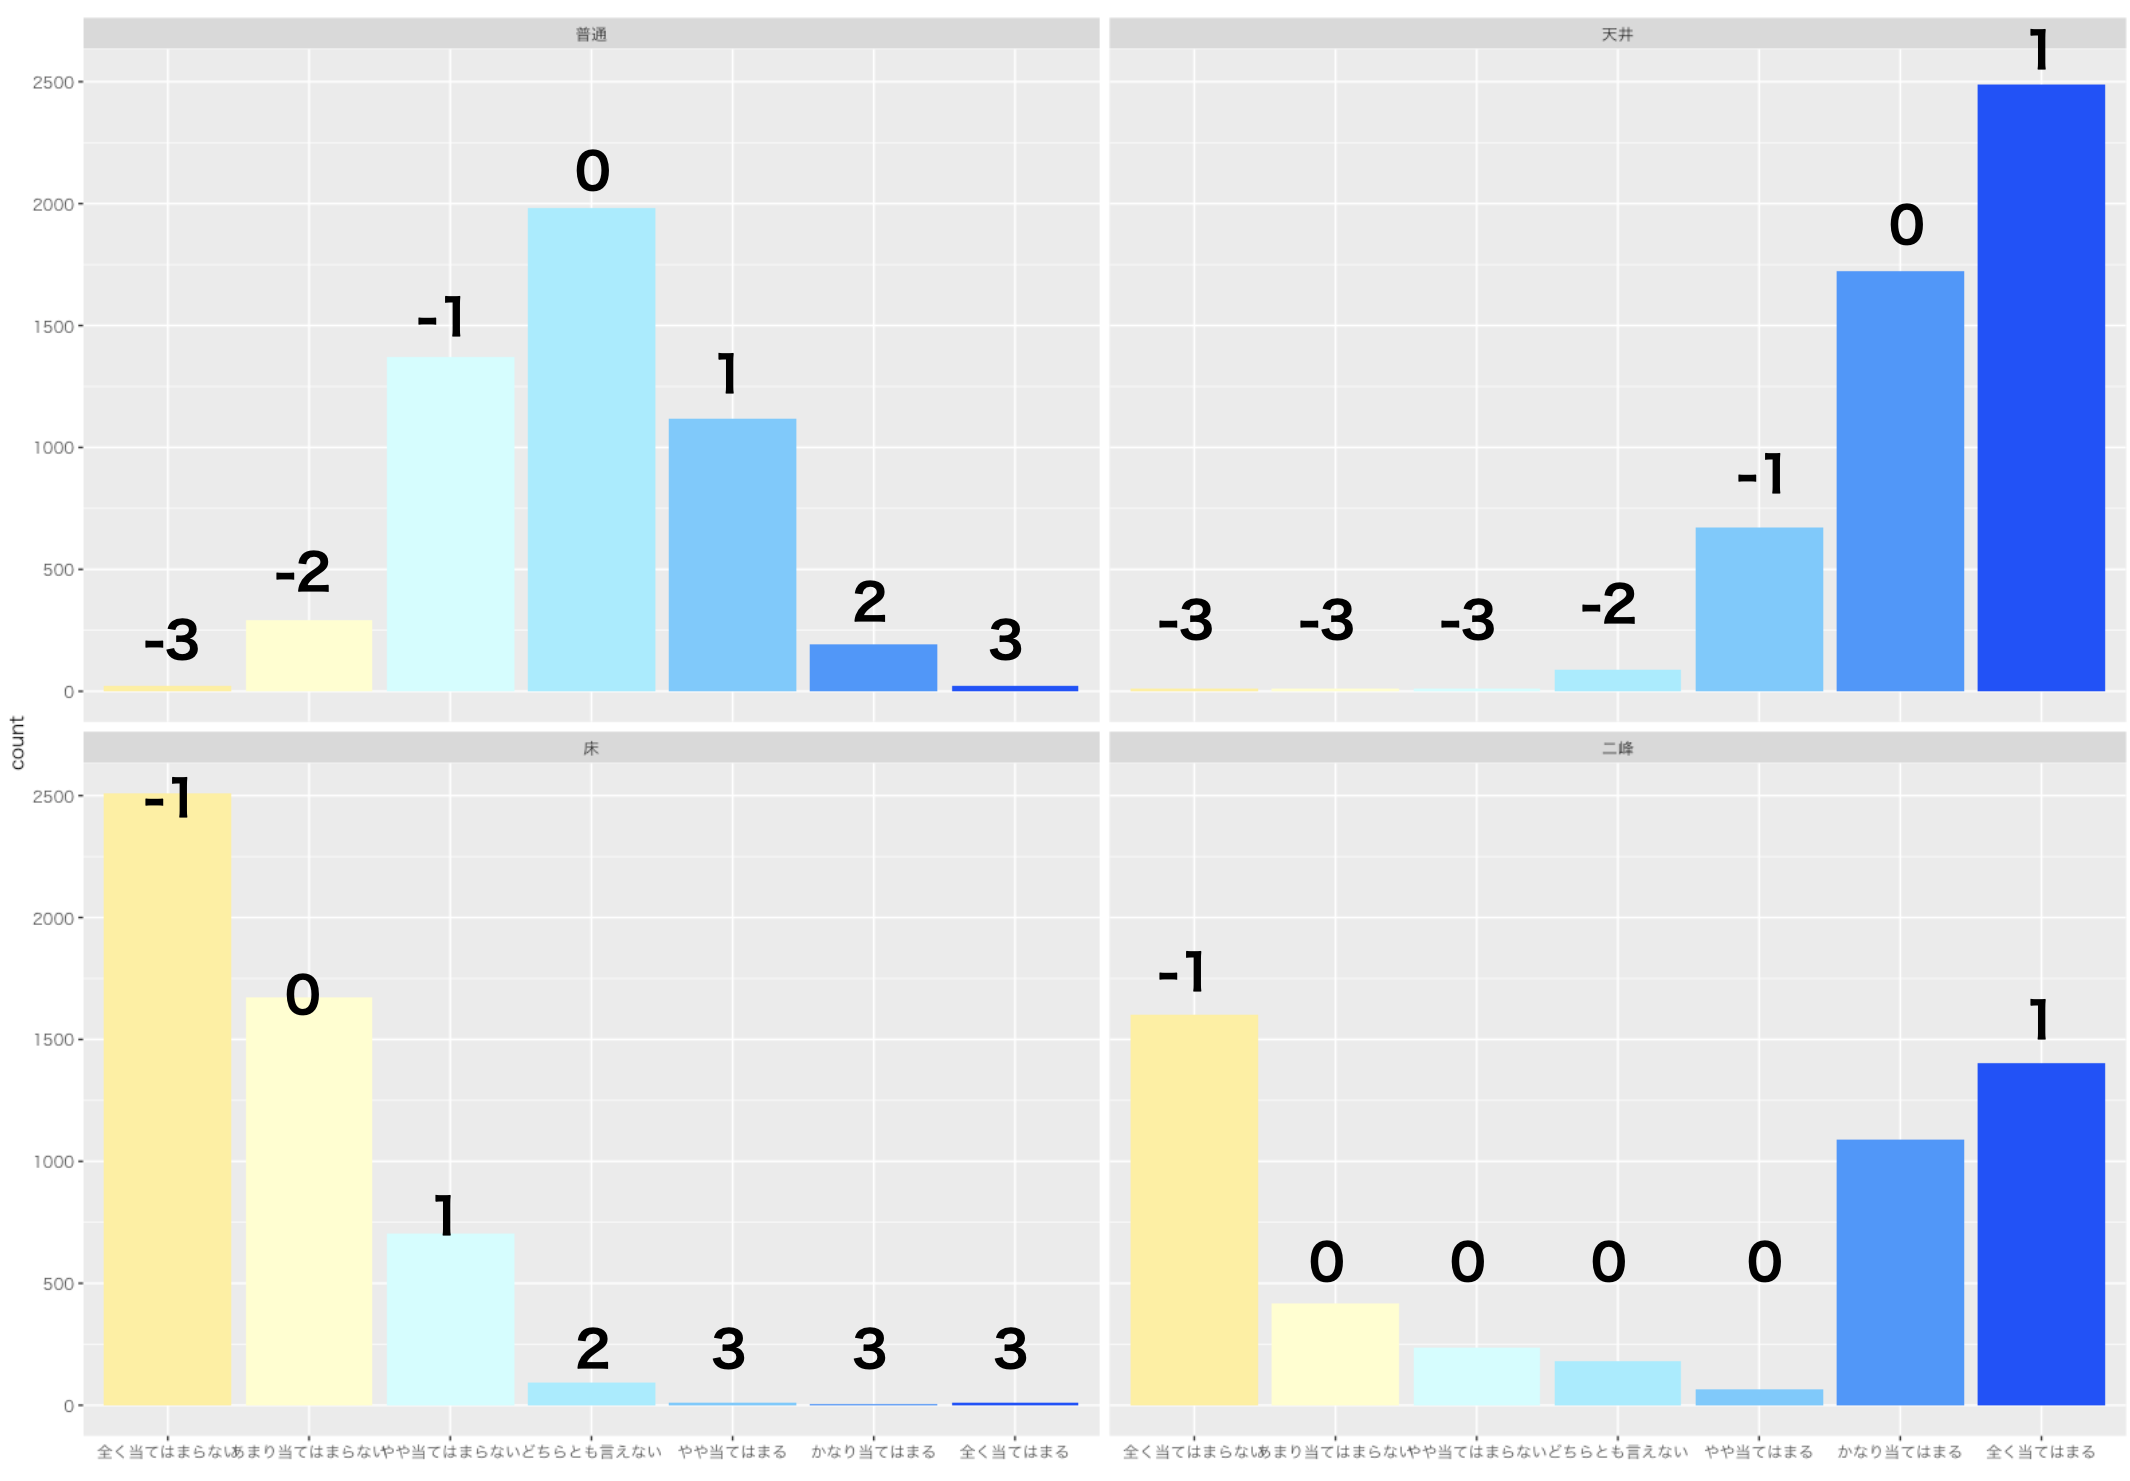
\includegraphics[width=0.8\linewidth,keepaspectratio,keepaspectratio,clip]{../images/02_scaling/LikertCeilFloor.png}
		\caption{天井効果・床効果の見られた尺度}
		\label{LikertCeilFloor}
	\end{center}
\end{figure}

また言葉で指示した他者・事象・現象が\kenten{同一のものであるかどうか}について，妥当性あるいは言語という共通基盤の頑健性について考えておく必要があります。社会的態度の研究の場合，たとえば政治的態度を研究するのことを考えたとしましょう。「自民党についての態度」を測定する場合，「自民党について」の意見が自分にどの程度当てはまるかを回答者個々人が判断することになりますが，このとき全員の頭の中に想定された「自民党」は同じ対象でなければなりません。日本における一般的な社会人であれば，「自民党」といえばあの自由民主党のこと，と誰でも同じものを思い浮かべられるでしょう。ここでアメリカの民主党を考えたり，イギリスの労働党を考えながら回答しているような人がいれば，回答パターンは無茶苦茶なものになってしまうでしょう。

しかし評価してもらう対象が「配偶者」「教師」「音楽」といったものであればどうでしょうか。誰1人として同じ配偶者を持っている人はいませんから，ある人のパートナーに対する態度と，別の人のパートナーに対する態度が同じもの(並べて，集計して，正規分布するもの)といえるでしょうか。「世話になった教師」といえば，ある時代のある学校においては「あの先生！」と特定できるかもしれませんが，それでも「自分は別の先生に世話になった」という人もいるでしょうし，時代と場所が変われば当然同じ人ではなくなります。「好きな音楽について」であっても，ロック，テクノ，K-Popなどなど，同じ「音楽」という括りで表現して良いものでしょうか。雅楽を想定している人と，パンクロックを想定している人が，「音楽とは穏やかな気持ちにさせてくれる」という意見に同じ次元で反応しているといえるでしょうか。

この批判はややもすると，言いがかりに聞こえるかもしれません。\kenten{「配偶者」「教師」という言葉で表される典型的なパターン}を研究したい，つまり言葉の使われ方の研究であれば問題ないかもしれません。あるいは社会通念上共通する架空の典型例，すなわち「あるある」ネタ研究であるなら，文化的な研究として価値があることかもしれません。しかし一人ひとりの主観的経験や心情を測定するというのとは，少し次元が違ってきているようです。

社会的態度は，個々人に数値を付与して個人間で相対的に比較することを可能にしてくれます。しかしそのことと，「その人が社会的態度を有している」かどうかについては，別の観点から考える必要もありそうです。このことについてはまた後で触れることになります。

\paragraph{他者や事象についての言及を，外的基準で評価する場合}
この領域は，事実の言語報告ですから，社会調査や実態調査として使われるところです。本人の言語報告に依存することなく，調べて裏取りをすることも可能ではありますが，「聞いた方が早い」から聞いているわけです。例えば家計収入など，本人の前年度の納税証明書を提示してもらえれば，円の単位まで正確に測定できますが，そこまでの精度や手間が必要ではないので「100万円未満，100〜200万円，200〜500万円・・・」等々の範囲で聞いていったりします。

プライベイトな情報であれば社会的望ましさの影響が，過去の記録を回顧して回答してもらう場合は記憶の歪曲といった問題が考えられますから，正しく事実を記録したいのであれば裏取りをするべきでしょう。言語による解答はあくまでも近似的，簡便的なスコアでしかないことに留意することが重要です。またこうした尺度で報告されるものは，調査前後の文脈によって大きく影響される可能性がありますから，「このような報告があるから」ということをエビデンスとするにはやや弱いかもしれない，と考えておいた方がいいかもしれません。

\subsection{心理尺度の限界}

見てきたように，リッカート法はサーストン法の簡易版であり，これらは社会的態度を測定するためのものでした。社会的態度には正規分布するという仮定があり，同様の仮定がたてられる性格心理学の領域などであれば，リッカート法のような目盛をつけることでの測定・数値化に根拠があると言えるでしょう。言い換えれば，分布の過程や回答パターンの累積が適切な操作でない場合，数値化の根拠がないとも言えます。
\underline{リッカート法は5，7段階の目盛を作ることではありません}。理論的前提が満たされない場合は使用を控えるか，異なる分析方法を考えるべきです。リッカート法で測定した変数は，因子分析法によって分析され，因子を見出して検討するというのがよく見られる手法ですが，実は数値化の根拠がない場合は，この分析方法の適用も間違っています。その分析法が使えないなら，多変量データは無用の長物か，というとそうではなくて，双対尺度法\parencite{Nishisato2010}や多次元尺度構成法\parencite{Takane198002}，クラスター分析\parencite{clusterAnalysis}など，数値化の理論に適した分析方法を使えば良いのです。これが使われていないのは，心理学者の不勉強としか言いようがないとおもいます。もちろん心理学者の研究の主眼は別にあって，分析法の理解に時間を費やしていられない，という反論があるだろうことは容易に想像できますが，だからと言って間違ったものを間違って分析していたのでは本末転倒ではありませんか。

これほど心理尺度が乱立した理由の一つは，この因子分析法がなんかカッコよかったこと，統計ソフトで誰でも簡単にその分析ができるようになったこと，が一因であるように筆者は考えています。かっこいいから，簡単だからという理由が，科学的な厳密性に依拠しないことはもちろんです。皆さんは周囲が統計ソフトで踊っている間に，しっかりと理論的な根拠と数理的な手続きを身につけ，正しく心理尺度が使えるようになってほしいと思います。


\section{課題}
\paragraph{リッカート法}シグマ法でなく機械的に数字を割り振るとどのような問題が生じるか，自分で数値例を作って検証してみてください。
\paragraph{信頼性の記述と報告}心理学の尺度作成に関する論文\footnote{日本心理学会が出している「心理学研究」という学会誌では，【資料】というカテゴリーで毎回のように新しい尺度が報告されています。}を読み，信頼性についてどのように記述されているかを確認してみましょう。
\paragraph{さまざまな妥当性}妥当性にはさまざまなものがあります。\textcite{kosugi2016b}などを参考に，妥当性について自分なりに調べてみてください。
\paragraph{リッカートのシグマ法} 表\ref{example2_1}のように，「かなり当てはまる」や「まったく当てはまる」など尺度の右の方に丸をつける人が多かった項目があったとします。この時の尺度値をリッカートのシグマ法に則って算出してみてください。

\begin{table}[ht]
	\centering
	\caption{天井効果の出た尺度}
	\begin{tabular}{rp{1cm}p{1cm}p{1cm}p{1cm}p{1cm}p{1cm}p{1cm}}
		\hline
		反応カテゴリ      & \pbox<t>{\small{まったく当てはまらない}} & \pbox<t>{\small{あまり当てはまらない}} & \pbox<t>{\small{やや当てはまらない}} & \pbox<t>{\small{どちらとも言えない}} & \pbox<t>{\small{やや当てはまる}} & \pbox<t>{\small{かなり当てはまる}} & \pbox<t>{\small{まったく当てはまる}} \\
		\hline
		出現度数        & 1.00                          & 3.00                         & 5.00                        & 18.00                       & 24.00                     & 53.00                      & 56.00                       \\
		相対度数        & 0.01                          & 0.02                         & 0.03                        & 0.11                        & 0.15                      & 0.33                       & 0.35                        \\
		累積相対度数      & 0.01                          & 0.03                         & 0.06                        & 0.17                        & 0.32                      & 0.65                       & 1.00                        \\
		累積相対度数の確率点  & -2.50                         & -1.96                        & -1.59                       & -0.96                       & -0.47                     & 0.39                       & $\infty$                    \\
		累積相対度数の確率密度 & 0.02                          & 0.06                         & 0.11                        & 0.25                        & 0.36                      & 0.37                       & 0.00                        \\
		\hline
	\end{tabular}
	\label{example2_1}
\end{table}

\end{document}
